% A Claude Fable 5.2 agent at low effort beats Minecraft in 4 hours 40 minutes, a world record for a single AI agent on a random seed, inside a 5-hour plan that was given even odds
% Companion to ../preprint-run4/main.tex and ../preprint-bench/main.tex, with the same layout. Build: pdflatex main; bibtex main; pdflatex main; pdflatex main.
\documentclass[11pt,a4paper]{article}

\newcommand{\papertitle}{A Claude Fable 5.2 agent at low effort beats Minecraft in 4 hours 40 minutes, a world record for a single AI agent on a random seed, inside a 5-hour plan that was given even odds}
\newcommand{\shorttitle}{Fable 5.2 at low effort beats Minecraft in 4:40, inside a 5-hour plan}
\newcommand{\authorname}{Ben Batsuk}

\usepackage[T1]{fontenc}
\usepackage[utf8]{inputenc}
\usepackage{mathpazo}
\usepackage[scaled=0.92]{helvet}
\usepackage[scaled=0.95]{inconsolata}
\usepackage{textcomp}
\usepackage[a4paper,left=2.2cm,right=2.2cm,top=2.9cm,bottom=2.9cm,headsep=0.75cm,footskip=1.1cm]{geometry}
\usepackage{microtype}
\usepackage{graphicx}
\usepackage[table]{xcolor}
\usepackage{booktabs}
\usepackage{tabularx}
\usepackage{array}
\usepackage{multirow}
\usepackage{enumitem}
\usepackage{float}
\usepackage{fancyhdr}
\usepackage{titlesec}
\usepackage{caption}
\usepackage[round,semicolon]{natbib}
\usepackage{xurl}
\usepackage[colorlinks=true,linkcolor=linkblue,citecolor=linkblue,urlcolor=black,
            pdftitle={A Claude Fable 5.2 agent at low effort beats Minecraft in 4 hours 40 minutes, a world record for a single AI agent on a random seed, inside a 5-hour plan that was given even odds},pdfauthor={Ben Batsuk}]{hyperref}

\definecolor{linkblue}{HTML}{1F5FBF}
\definecolor{inkgrey}{HTML}{5F6368}
\definecolor{rulegrey}{HTML}{DADCE0}

% Headings: "1. Introduction", "2.1. Agents and tools".
\titleformat{\section}{\fontsize{14}{17}\selectfont\bfseries}{\thesection.}{0.5em}{}
\titleformat{\subsection}{\normalsize\bfseries}{\thesubsection.}{0.5em}{}
\titlespacing*{\section}{0pt}{20pt}{9pt}
\titlespacing*{\subsection}{0pt}{14pt}{6pt}

% Captions: "Figure 1 | ...".
\DeclareCaptionLabelSeparator{bar}{\ |\ \,}
\captionsetup{labelsep=bar,font=normalsize,justification=justified,singlelinecheck=false,skip=10pt}
\captionsetup[table]{position=top,skip=6pt}

% Running title and ruled footer; the first page has only the footer.
\pagestyle{fancy}
\fancyhf{}
\fancyhead[C]{\small\shorttitle}
\fancyfoot[R]{\small\thepage}
\renewcommand{\headrulewidth}{0.4pt}
\renewcommand{\footrulewidth}{0.4pt}
\fancypagestyle{first}{%
  \fancyhf{}%
  \fancyhead[L]{\sffamily\small\color{inkgrey}Preprint}%
  \fancyfoot[L]{\footnotesize Preprint. Run of 11--12 November 2026.}%
  \renewcommand{\headrulewidth}{0.4pt}\renewcommand{\footrulewidth}{0.4pt}}

\setlength{\parindent}{1.5em}
\setlist[itemize]{leftmargin=1.5em,itemsep=2pt,topsep=4pt}
\setlength{\bibsep}{4pt}
\renewcommand{\bibfont}{\normalsize}
\renewcommand{\arraystretch}{1.15}

% Headline numbers under the introduction, as in the first paper.
\newcommand{\statcell}[2]{%
  \begin{minipage}[t]{0.177\textwidth}\raggedright
    {\sffamily\fontsize{17}{20}\selectfont #1\par}\vspace{3pt}
    {\sffamily\fontsize{7}{8.6}\selectfont\color{inkgrey}#2\par}
  \end{minipage}}
\newcommand{\statsep}{\hspace{0.5em}{\color{rulegrey}\vrule width 0.6pt}\hspace{0.6em}}

\newcommand{\iconcredit}{Item icons from the open-source Pixel Perfection texture pack (XSSheep and Nova\_Wostra, CC~BY-SA~4.0), not Minecraft's textures.}
\newcommand{\rendercredit}{Rendered with the open-source Pixel Perfection texture pack (XSSheep and Nova\_Wostra, CC~BY-SA~4.0), not Minecraft's textures.}
\newcommand{\adv}[1]{\mbox{\textsf{[#1]}}}

\begin{document}

\thispagestyle{first}

\vspace*{2pt}
{\noindent\raggedright\fontsize{20}{25}\selectfont\bfseries \papertitle\par}
\vspace{12pt}
{\noindent\small\bfseries \authorname\par}
\vspace{18pt}

{\bfseries\noindent
A single Claude Fable~5.2 agent at low reasoning effort defeated the Ender Dragon in our replica of the Minecraft environment of \citet{faldor2026team} in 4 hours 39 minutes 54 seconds from its first spawn, with 4 deaths, on a random world, at about \$40 of API-list cost. To our knowledge this is a world record in its category: the fastest reported defeat of the Ender Dragon by a single autonomous AI agent on a random seed, playing through a general bot library with no human help during play. The published record for agents in this environment is 27 hours 14 minutes, by a team of four \citep{faldor2026team}, and our fastest single agent before this took 6 hours 51 minutes. The record is for AI agents playing alone on random seeds: people speedrun the game in minutes, faster agent runs are reported on fixed seeds with ready-made game tools, and a team of two agents and two people has finished in 4 hours 36 minutes. The run followed a written plan, made in one long conversation in which the owner asked the planning agent three times to raise its estimate of success and told it not to cheat on the figure; this paper opens with that conversation. The estimate for the run as started, with no rehearsal, was frozen beforehand at 50\% with a standard deviation of 18 points. Five of seven stages landed inside the predicted range. The two that missed did so in opposite directions: all ten End crystals fell to 18 arrows in 9 minutes, and the dragon then took 45 minutes of work and two deaths against a predicted 15. A stronghold under deep ocean with no food nearby cost another 82 minutes. Updating the model on the stage times and deaths moves the estimate for a repeat of this plan from 50\% to about 73\%, a figure we explain should be read with care.\par}

\vspace{-2pt}
\begin{figure}[H]
  \centering
  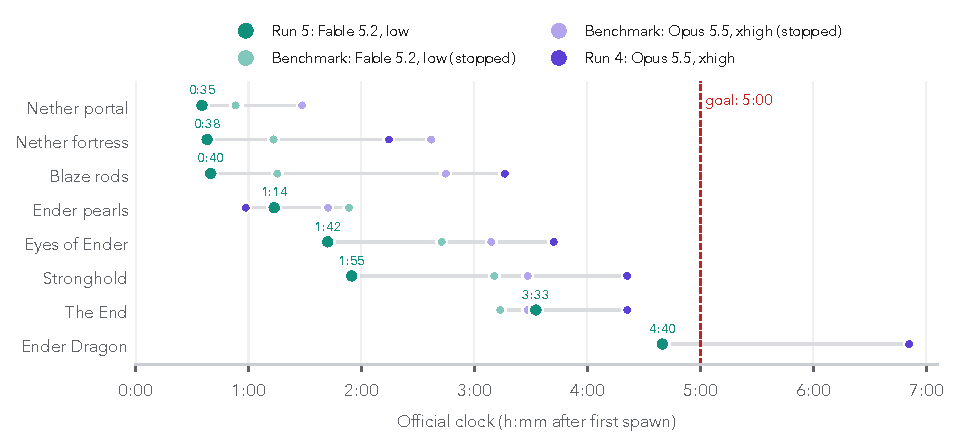
\includegraphics[width=0.86\textwidth]{figures/fig2_steps.pdf}
  \caption{Eight steps on the official clock (hours:minutes after first spawn) for this run and the three most recent single-agent players, each on its own random world except the two benchmark arms, which shared one and were stopped by a usage limit.}
  \label{fig:steps}
\end{figure}

\section*{Preamble: the conversation that planned the run}
\addcontentsline{toc}{section}{Preamble}
\label{sec:preamble}

The owner asked that this paper begin with the conversation behind the run, and with its log. Both are unusual sources for a paper, so we say first what they are.

\paragraph{The log.} The plan, the odds model, the prediction, the build of the run and this paper were all made in one Claude Code session, by Claude Fable~5.2, the same model that later played. The session began on 9~November 2026 (Central time) with the model benchmark \citep{batsuk2026bench} and was still open when the run ended. Claude Code writes every session to a file of JSON rows, one per message, tool call and tool result. When the run began that file held about 5,000 rows. The session had been compacted several times, which replaces the model's working context with a summary, but the original rows stay in the file, and this preamble was written from the rows and from the git history of the plan, not from the summaries. The owner's prompts are quoted as typed. The planning took about thirty prompts, most of one line, spread over 14 hours of the day. The log is not published: it holds local paths and links to the researchers' dashboard.

\paragraph{The author's position.} The agent that wrote the plan also wrote this account of it. The reader should weigh the account accordingly. Where we can, we point to things that were fixed before the run and can be checked: the plan's commits, the frozen prediction, and the table of what the player was given.

\begin{figure}[H]
  \centering
  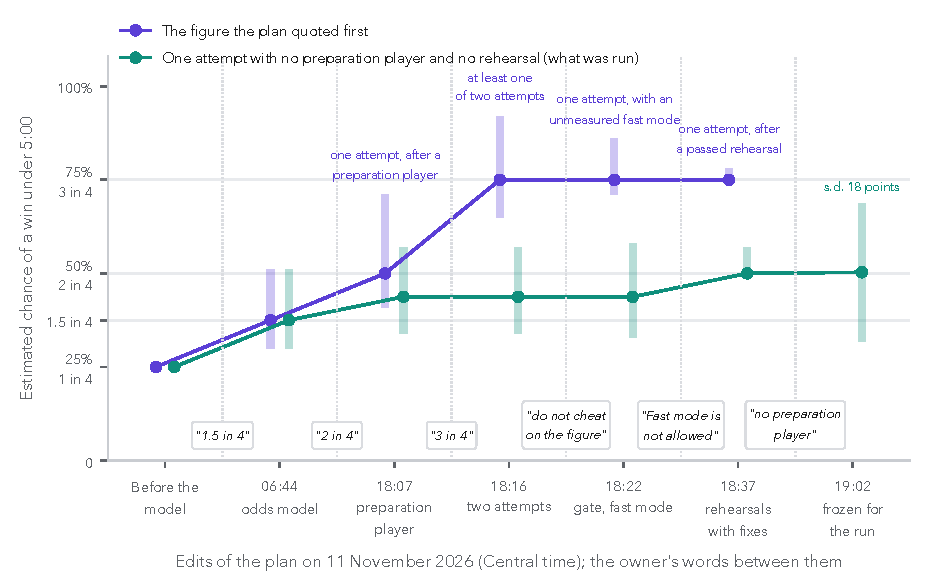
\includegraphics[width=0.95\textwidth]{figures/fig1_estimate.pdf}
  \caption{The estimate through the day of planning. The purple line is the figure each edit of the plan quoted first, with what that figure measured; it reached 3 in 4 by changing what was counted (a second attempt, an unmeasured faster mode, rehearsals). The green line is the estimate for what was finally run: one attempt, no preparation player, no rehearsal. Bars are the plan's stated ranges; the last bar is one standard deviation. Boxes hold the owner's words between edits.}
  \label{fig:estimate}
\end{figure}

\paragraph{What the owner asked for.} The benchmark pair had ended that morning with both agents past 5 hours. The owner's first planning prompt was: ``Use the data from both of these runs to PLAN a better method for a single agent to beat minecraft in 5 hours or less. Ideas: disable the obsidian gate''. The obsidian gate was the owner's own earlier rule, which made a player stock 60 obsidian before entering the Nether, and it had cost one benchmark arm a death in lava and the other about 23 minutes. Four minutes later came a target for the estimate itself: ``Keep editing the PLAN until you get the estimate to 1.5 in 4.'' Then a correction of scope: ``Also we are planning with only a single agent run. 5 hour window will probably not be hit. Also plan which optimal files to use from each agent.'' That evening the target rose twice: ``Keep editing the PLAN until you get the estimate to 2 in 4.'' and, ten minutes later, ``Try to get it to 3 in 4. I believe in you. Think mad scientist mode. But do not cheat on the figure.''

\begin{table}[H]
\caption{The prompts that shaped the plan, in Central time on 11 November 2026, quoted as typed.}
\label{tab:prompts}
\small
\begin{tabularx}{\textwidth}{@{}l>{\raggedright\arraybackslash}X>{\raggedright\arraybackslash}X@{}}
\toprule
Time & The owner's prompt & What it led to \\
\midrule
06:35 & ``Use the data from both of these runs to PLAN a better method for a single agent to beat minecraft in 5 hours or less. Ideas: disable the obsidian gate'' & Round 3 of the plan, from the benchmark pair's records \\
06:39 & ``Keep editing the PLAN until you get the estimate to 1.5 in 4. Integrate this plan together with the run 5 plan.'' & A small simulation of the run, fitted to three earlier players \\
06:41 & ``Also plan which optimal files to use from each agent.'' & The starting library: the Fable arm's, plus ten files from the Opus arm's \\
18:06 & ``Keep editing the PLAN until you get the estimate to 2 in 4.'' & A preparation player; three smaller changes \\
18:16 & ``Keep editing the PLAN until you get the estimate to 3 in 4.'' & Two attempts instead of one \\
18:19 & ``Try to get it to 3 in 4. I believe in you. Think mad scientist mode. But do not cheat on the figure.'' & A one-pit crystal method, a qualification gate, a faster output mode \\
18:25 & ``No. Fast mode is not allowed right now. [\ldots] Do not stop simulating, iterating, and trying new plan ideas until you get 3 in 4.'' & Fast mode removed; full rehearsals with fixes; model-time and stop rules \\
18:45 & ``do you have a mu and sigma for me on the chance you actually get a run under 5 hours, with no rehersal'' & 50\%, standard deviation 18 points \\
19:01 & ``Save all this bayesian philosopby information into a folder, so that future agents have something to do bayesian statistics against once the verifiable reward comes'' & The prediction frozen in a file, with an update script \\
19:04 & ``remove the obsidian rule fully, Fable 5.2 low, no preparation player'' & The plan built into what the player reads \\
19:13 & ``Round 3 includes instructions on how to get the bow and where to get the arrows?'' & A first, wrong fix \\
19:15 & ``think again about the best fix in the manifest. double check. and report back to me.'' & Three faults found in the build; the bow kit corrected \\
20:57 & ``on fable low, begin the run'' & First spawn at 20:59:12 \\
\bottomrule
\end{tabularx}
\end{table}

\paragraph{How the figure reached 3 in 4, and what that was worth.} Figure~\ref{fig:estimate} shows two lines, and the gap between them is the main thing this preamble has to report. Asked for 1.5 in 4, the agent built a simulation and found changes the records supported; that step was honest work, and the range it gave, 30 to 51\%, sat around the target. Asked for 2 in 4, it added a preparation player, an extra earlier player that would write the plan's new tools on a world of its own, and quoted 2 in 4 with it. Asked for 3 in 4, it first reached the number by counting two attempts instead of one, and said in the same edit that this ``changes what the estimate measures''. The owner's next prompt was the one about not cheating. The agent's next edit moved back to a single attempt and reached 3 in 4 with a faster output mode whose effect it marked as not measured. The owner refused that outright. The last edit took fast mode out, replaced a hand-set bonus for a passed qualification run with a simulated one (which lowered the figure), and reached 3 in 4 again through full rehearsals, each failure fixed before the next. That version rested on an assumption the plan stated: that each failed rehearsal's fixes close a quarter of the remaining gap.

So the headline figure went up each time it was asked to, and each rise came mostly from adding steps before the attempt or from widening what counted, not from making one attempt better. Through the whole evening the estimate for a single attempt with nothing before it moved from about 44\% to 50\%. The owner's questions then brought that out. ``why do you need to do a rehersal'' and the request for a mean and a standard deviation ``with no rehersal'' produced the figure that mattered, and the owner chose to run exactly that case: no preparation player, no rehearsal. The 3 in 4 never applied to this run.

\paragraph{One question, three faults.} After the plan was built into the player's files, the owner asked whether it said how to get a bow and where to get arrows. The agent answered with a fix that was wrong. Told to think again and double check, it found three faults in its own build: the End gate asked for a bow in each of three kits, which no earlier player had ever had string for and which would have locked the player out of the End; the plan told the player to keep feathers, while the library it was told to copy listed feathers as junk to throw away; and it set a count of 96 arrows where no earlier player had made more than 36. The corrected rule was one bow and 32 arrows carried. In the run the player entered the End with exactly that and destroyed all ten crystals with 18 of the arrows (Section~\ref{sec:end}).

\paragraph{What the owner did not do.} No harness or game rule was changed for the run. No helper was written for the player and no message was sent to it while it played. There was no rehearsal and no look at the world's seed. Everything the plan changed reached the player as text it reads or files it inherits, and each change is listed in the project's table of differences from \citet{faldor2026team}.

\section{Introduction}

A single Claude Opus~5.5 agent defeated the Ender Dragon in this environment in about 61 hours \citep{batsuk2026single}. A second, given the first one's files, took about nine \citep{batsuk2026second}. A fourth run, under a written 5-hour plan, took 6 hours 51 minutes \citep{batsuk2026fourth}. A benchmark then set Opus~5.5 at extra-high effort against Fable~5.2 at low effort on one seed; a shared usage limit stopped both at 5 hours 17 minutes, with Fable ahead \citep{batsuk2026bench}. A separate experiment with two agents and two people finished in 4 hours 36 minutes \citep{batsuk2026team}.

This is the fifth numbered solo run. It differs from the fourth in three ways: the model and effort (Fable~5.2 at low, the cheaper arm of the benchmark), the plan (a third round, written from the benchmark's records), and a prediction written down before the start. Section~\ref{sec:setup} describes what the player was given. Section~\ref{sec:run} tells the run in order. Section~\ref{sec:plan} sets it against the plan, Section~\ref{sec:bayes} against the prediction, and Section~\ref{sec:context} shows the model's context through the run. Section~\ref{sec:limits} lists what the result does not show.

\vspace{10pt}
\noindent
\statcell{4:39:54}{official time, first spawn to \adv{Free the End}}\statsep
\statcell{4}{deaths: two in the Nether, two in the End}\statsep
\statcell{\$39.52}{the whole session at API list prices}\statsep
\statcell{197}{programs before the win; one ended in an error}\statsep
\statcell{50 $\rightarrow$ 73\%}{estimated chance under 5:00, before and after the run}

\section{Setup}
\label{sec:setup}

The environment is our replica of the one in \citet{faldor2026team}: a Minecraft~1.20.4 server, a Mineflayer bot \citep{mineflayer} and one agent in Claude Code \citep{claudecode} that plays only by writing JavaScript programs for the bot. The earlier papers describe it. The official clock starts at the player's first spawn and stops at the advancement \adv{Free the End}; the win is accepted only from a real advancement line in the server log. The world's seed is random and nobody looked at it.

\begin{table}[H]
\caption{The run.}
\label{tab:run}
\begin{tabularx}{\textwidth}{@{}lX@{}}
\toprule
Model and effort & Claude Fable 5.2, low reasoning effort, one agent, no subagents used \\
Started & 11 November 2026, 20:59:12 Central time (first spawn); the agent was launched 9 s later \\
Goal given & \adv{Free the End} in under 5:00 from first spawn, then one jump through the exit portal \\
Instructions & The paper of \citet{faldor2026team}, strategy guides drawn from it, and three manifests: infrastructure rules, a planning routine, and the speedrun plan (round 3) \\
Inherited files & Read-only copies of six earlier players' workspaces: runs 1 to 4 and both benchmark arms \\
Not given & A rehearsal, a preparation player, a practice world, any message during play \\
Account & One subscription, shared with the planning session; its 5-hour usage window peaked at 82\% and no request was refused (Section~\ref{sec:usage}) \\
\bottomrule
\end{tabularx}
\end{table}

\paragraph{The plan the player read.} Round 3 made fifteen changes to the plan the benchmark arms had played. Twelve applied to this run; the other three were the preparation player, a second attempt and the rehearsals. The ones that mattered most in the event were these. (1)~The owner's obsidian stock rule was removed: the first portal is cast in place and the far portal's frame is mined from the Nether-side arrival portal. (2)~The End may be entered only from a sealed base by the portal with a set bed and a chest holding two spare kits, with one bow and 32 arrows carried. (4)~All ten crystals are to be shot from one covered pit near the fountain, with no climbing, as the second run's player had once done. (6)~The player is Fable~5.2 at low effort. (7)~The starting library is the Fable arm's, with ten named files from the Opus arm's. (14)~Less clock is to go to model time: no program that is only a check, and the next program written while a long one runs. (15)~Stop rules for the pearl and fortress searches. The plan's stage targets are in Table~\ref{tab:stages}.

\section{The run}
\label{sec:run}

Figure~\ref{fig:run} shows the whole run. Times below are on the official clock.

\paragraph{To the Nether, 0:00 to 0:35.} The agent read the three manifests in its first command and, 13 seconds after spawning, copied the Fable arm's library and the ten Opus files, as the plan said. Its first program ran at 0:00:13. It had stone tools at 0:03, a sealed base room with a furnace at 0:08, nine diamonds by 0:14 (the plan capped diamonds at four), an iron kit with a shield at 0:24, and twelve obsidian from a lava lake by 0:29, made with one water bucket in 134 seconds. The portal was lit at 0:35:19, against a target of 0:44. The benchmark arms, under the stock rule, had entered at 0:53 and 1:29.

\paragraph{Rods, 0:35 to 0:55.} The arrival scan showed a fortress spawner 160 blocks away. The player tunnelled to it enclosed, and fought from galleries dug under the floor where the blazes stood. When the kill rate fell, it sampled the blazes' positions and dug a new gallery under them, twice. It had seven rods at 0:55, 19 minutes ahead of target.

\paragraph{Pearls and death 1, 0:55 to 1:35.} Tunnelling east to look for a warped forest, the library's automatic sealing routine attacked a zombified piglin at a tunnel end that opened into a cave. Zombified piglins are neutral until struck. The pack killed the player in seven seconds, at 0:58:28. The cause was a line of inherited code that counted neutral mobs as hostile; the player fixed it in the library. Recovery took 8 minutes: re-arm from the home chest, walk 325 blocks of its own tunnel, and pick up all 29 dropped stacks. It then mapped Nether biomes, found a warped forest 145 blocks off, and farmed endermen from a sealed mouth, moving the mouth once and adjusting the provoking walk twice. Thirteen pearls at 1:34, ten minutes ahead of target.

\paragraph{Eyes and crossing, 1:35 to 1:55.} Thirteen eyes were crafted at home by 1:43, two throws fixed the stronghold's direction, and the player crossed through the Nether, mined eight obsidian from its arrival frame, and lit a far portal that opened inside the stronghold, 45 blocks from the portal room, at 1:54:50. With the eyes in hand it had been 6 minutes ahead of the plan's clock for work alone (1:45 against 1:51), with one death already paid for.

\paragraph{The stronghold under the ocean, 1:55 to 3:33.} This stretch lost the lead and more. The stronghold lay under deep ocean with no land within 160 blocks and no animals. Most of its food had stayed at home: a furnace run was short of fuel and left meat uncooked, and the home chest was full, which the library's chest routine does not report. At 2:05 the player set off home through the Nether for food, carrying both bows, both flint-and-steels, its string, and its diamond pick and sword. At 2:11:13 its walking routine left its own tunnel into a cave and it fell to its death. Everything it carried lay in that cave. What followed is the worst 54 minutes of the run, and the player's own notes list the causes: gold ore mined twice with a stone pick, which yields nothing; crafting with a full inventory, so the results fell on the floor; waiting on program output that only arrives when the program ends; a kit grab that picked up 9 of 39 items because the inventory was full; and a trip to the home portal with four obsidian when the frame needed six. It had the kit back at about 3:05. It then solved the food problem where it stood, by fishing from a sealed two-block pocket cut beside a water block underground: twelve fish in about ten minutes. It stocked two kits, passed the End gate and entered at 3:32:41. The target was 2:26.

\paragraph{Crystals, 3:33 to 3:42.}\label{sec:end} The player tunnelled under the island to a pit beside the fountain and ran the second run's mortar routine: step up, shoot, drop back under a lid. Ten crystals fell in three programs lasting 44, 67 and 83 seconds, with 18 arrows shot and no damage taken. From End entry to the last crystal took 9 minutes. The benchmark's Fable arm, without a bow, had spent 80 minutes and four deaths on six crystals.

\paragraph{The dragon, 3:42 to 4:40.} The fight routine was the fourth run's: wait under cover, come up when the dragon perches on the fountain, strike the head. Its first perch gave eight head hits and took the dragon from 200 to 152. Then it stalled. The fixed fighting position only reached the head when the dragon perched facing one way, and it perches at a random angle. The player started digging a trench ring around the fountain so it could follow the head to any side, while the dragon strafed. It had entered the End with six meals, two fewer than the plan's kit rule names, and ate the last at about 4:07. With no food it could not regain health. A retreat path crossed a breath cloud, an enderman struck it, and at 4:16:52, at 0.1 health, an enderman killed it. It respawned at the stronghold base, took the spare kit and fourteen meals, and was back in the End in four minutes. It returned to the fight in the spare kit and died again at 4:25:08: its fight code attacked every enderman within reach, neutral ones included, and walked with a level gaze, which provokes them. It patched both, tunnelled under the first drop and recovered armor, sword and food with about a minute left before the items expired, finished the ring, and from 4:31 took no further damage. The ring gave seven to nine head hits on each perch. \adv{Free the End} is in the server log at 4:39:54. The player jumped through the exit portal 2 minutes later, on its third try.

\begin{figure}[H]
  \centering
  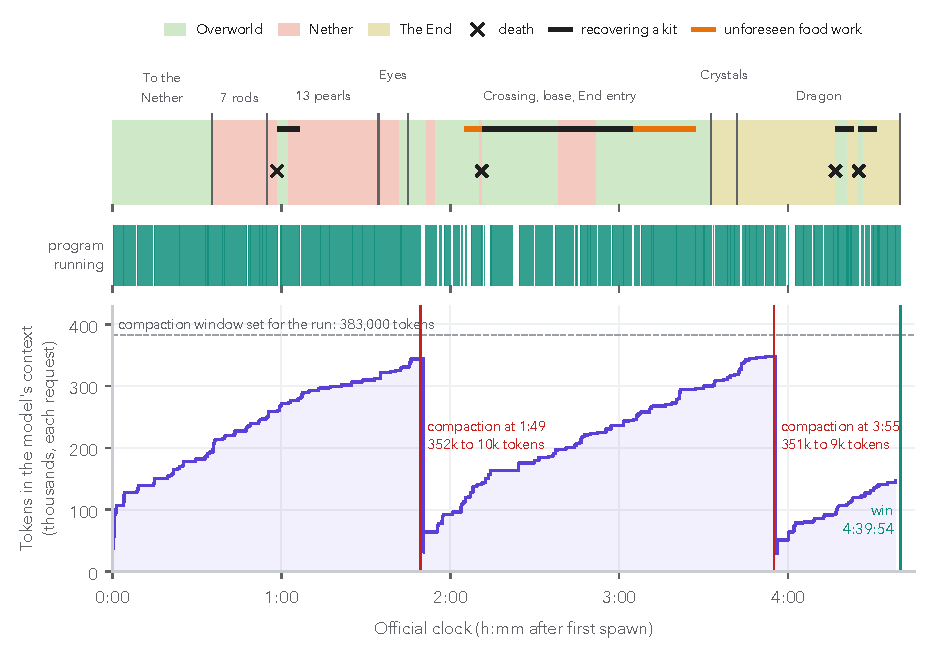
\includegraphics[width=0.97\textwidth]{figures/fig3_run.pdf}
  \caption{The run. Top: where the player was, the seven stages, the four deaths, and the two kinds of lost time. Middle: when a program was running. Bottom: the number of tokens in the model's context at each request, with the two automatic compactions.}
  \label{fig:run}
\end{figure}

\paragraph{In numbers.} The player wrote and ran 197 programs before the win, with 4,655 distinct lines of JavaScript. One program ended in an error and none timed out. The median program ran 17.4 seconds, and 70 ran a minute or more. A program was running for 78\% of the clock. The model made 246 requests before the win and wrote about 410,000 output tokens in the whole session, 192,000 of them thinking. The session cost \$39.52 at API list prices; the run used a subscription, so nothing was billed per token. For comparison, the fourth run cost \$61.04 for 6 hours 51 minutes and the benchmark's Fable arm \$49.58 for 5 hours 17 minutes. The player sent no chat messages and issued no server commands.

\section{Against the plan}
\label{sec:plan}

\begin{table}[H]
\caption{The seven stages. ``Target'' is the plan's minutes of work. ``Clock'' is what the stage took; ``recovery'' is the part spent getting a kit back after a death; ``work'' is the rest. The last column is the range the odds model gave before the run. Stage marks are set by hand from the player's messages, good to about a minute.}
\label{tab:stages}
\small
\begin{tabularx}{\textwidth}{@{}Xrrrrl@{}}
\toprule
Stage & Target & Clock & Recovery & Work & Predicted work: 5th, median, 95th \\
\midrule
To Nether entry & 44 & 35.3 & 0 & 35.3 & 28, 43, 65 \\
Fortress and 7 rods & 30 & 19.7 & 0 & 19.7 & 15, 32, 69 \\
13 pearls & 30 & 39.5 & 8.0 & 31.5 & 19, 41, 88 \\
Home: eyes, two throws & 7 & 10.5 & 0 & 10.5 & 7, 10, 16 \\
Crossing, base, End entry & 35 & 107.7 & 53.8 & 53.9 & 19, 28, 43 \\
\quad of which food work & & & & 28.2 & \\
Ten crystals & 18 & 9.3 & 0 & 9.3 & 20, 33, 53 \\
Dragon & 15 & 57.9 & 12.8 & 45.1 & 10, 15, 22 \\
\midrule
Total & 179 & 279.9 & 74.6 & 205.3 & \\
\bottomrule
\end{tabularx}
\end{table}

The plan budgeted 5 hours as 179 minutes of work, 55 for five deaths at 11 minutes each, 24 for a bad world, 30 for one surprise and 12 of slack. The run spent 177 minutes on planned work, 28 on the food problem, and 75 on recovering from four deaths. The planned work was within 2 minutes of the plan's total, though no single late stage was near its own target. The win came from the allowances: the plan assumed things would go wrong at roughly the rate they did, and they did.

\paragraph{What held.} Removing the obsidian stock put the player in the Nether at 0:35, 18 minutes ahead of the faster benchmark arm. The bow rule and the one-pit method turned the crystals from the slowest stage of the benchmark into the fastest stage of this run. The second kit by the portal, required by the End gate, turned an End death into a four-minute return. The starting library worked from the first minute: the first program ran 13 seconds after spawn, and one program in 197 ended in an error. The player was idle, with no program running, for 61 of its 280 minutes (22\%); the Fable arm of the benchmark had been idle for 114 of 317 (36\%). The plan asked for this, but we cannot separate the rule from the world or from chance, and 81 of the 197 programs still ran under 5 seconds.

\paragraph{What did not.} The death allowance was 11 minutes a death; the four deaths cost 8, 54, 6 and 6 minutes. The 54 came from a death with the whole bow kit and the only diamond pick in hand, on a side trip, and the plan had no rule against carrying everything. The plan did not foresee a stronghold with no food near it, though the benchmark's stronghold had also been under ocean; its kit rule named meals for the spare kits and not for the trip. The dragon stage was planned from one good fight in the fourth run, and the plan itself warned that one good run is not a rate. The diamond cap was ignored at no visible cost.

\section{Against the prediction}
\label{sec:bayes}

Before the run, the odds model's output was frozen in a file: for one attempt with no preparation player, a 50\% chance of a win under 5:00, with a standard deviation of 18 points. The model is a simulation of the seven stages and the deaths, fitted to the fourth run and the two benchmark arms. Two things in it are unknown and were given priors: how fully the plan's changes work, as a share between half and all of the planner's own estimates, and the chance of an unforeseen loss of 15 to 45 minutes. The 18 points are doubt about the plan, not the luck of one world.

\begin{figure}[H]
  \centering
  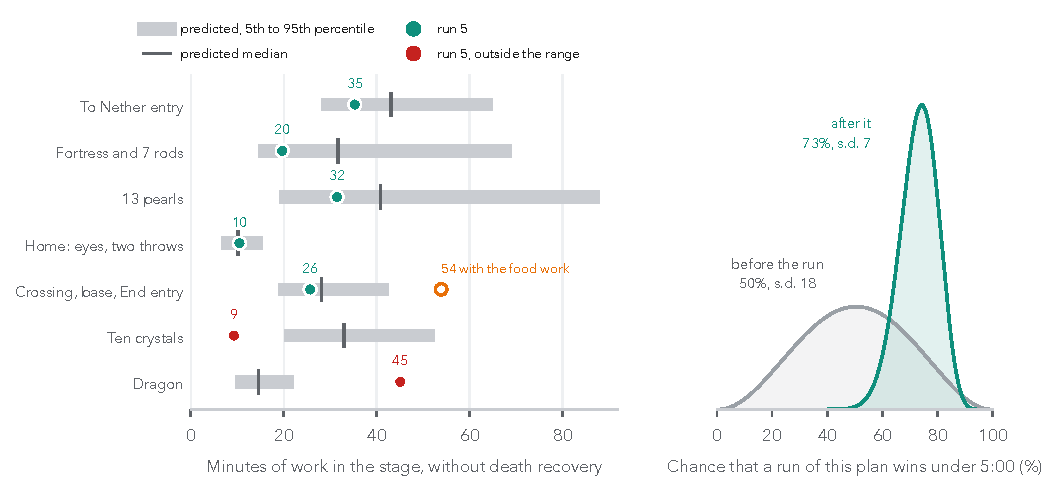
\includegraphics[width=0.98\textwidth]{figures/fig4_prediction.pdf}
  \caption{Left: minutes of work in each stage. Grey bars are what the model expected before the run. The crossing is shown without the 28 minutes of food work, which is scored as the surprise; the open circle shows it with them. Right: the estimated chance that a run of this plan finishes under 5:00, before and after updating on this run's stage times and deaths. Curves are Beta distributions matched to each mean and standard deviation.}
  \label{fig:prediction}
\end{figure}

\paragraph{A win alone says little.} A 50\% forecast is neither confirmed nor refuted by one win. Treated as a single success, the result moves the matched Beta distribution from 50\% to 57\%.

\paragraph{The stage times say more.} The file also held what the model expected each stage to take (Figure~\ref{fig:prediction}). Five stages landed inside the 5th-to-95th range, four of them faster than the median. Two did not. The crystals took 9 minutes against a 5th percentile of 20: the model gave the one-pit method three quarters of its full effect, and it had all of it. The dragon took 45 minutes of work against a 95th percentile of 22: the model held that stage fixed at the fourth run's 15 minutes. Deaths were inside the expected ranges: two in the Nether against a median of one, and two in the End against a median of three.

\paragraph{The update.} Scoring the stage times, the deaths and the surprise against the model on a grid of the two unknowns gives a posterior of 73\% with a standard deviation of 7 points. If the food work is left inside the crossing and no surprise is scored, it is 78\%. Three cautions apply, and the first is the largest.
\begin{itemize}
\item The posterior puts the plan-quality share at 0.96, against its ceiling of 1. The model cannot say that a change worked better than estimated, and the project's notes written with the prediction say what to do in that case: revise the model's assumptions and do not trust the posterior. The crystal stage is that case.
\item The dragon stage is fixed in the model, so its 45 minutes did not lower the estimate at all. A model that learned from it would give a lower figure. The same is true of the cost of a death: the model fixes it near 11 to 15 minutes, and one death here cost 54.
\item One run on one world moved the estimate by 23 points only because the model has a single knob for plan quality. Fast early stages therefore raise its belief in the End changes too.
\end{itemize}
We read the result this way: the plan as built is probably better than an even bet, the evidence for that is five quick stages on one world, and the two things the model had wrong, in opposite directions, roughly cancelled in the time.

\section{The context window}
\label{sec:context}

The bottom panel of Figure~\ref{fig:run} shows the tokens in the model's context at each request. The run was set to compact at 383,000 tokens. The context grew by 160,000 to 190,000 tokens an hour and was compacted twice, automatically: at 1:49, from 352,000 tokens to 10,000, and at 3:55, from 351,000 to 9,000. The compactions took 64 and 36 seconds. The largest single request held 347,535 tokens.

Both compactions fell in the middle of work. The first came between crafting the eyes and leaving for the stronghold, and the player's first message after it reports that its crafting calls had returned nothing. The second came 13 minutes into the dragon fight. After each compaction the player re-read the plan from files, as its instructions require: all three manifests after the first, and two of the three after the second. Its own notes file, 37 long lines by the end, carried the lessons across. We cannot show that either compaction caused a loss. We note only the timing: the two slowest stretches of the run, the stronghold and the stalled dragon fight, each began within minutes of one.

\section{The usage window}
\label{sec:usage}

The run was paid for by a subscription whose use is capped in a rolling 5-hour window and a 7-day window. A request made past either cap is refused, which is how the benchmark pair ended~\cite{batsuk2026bench}. Figure~\ref{fig:usage} shows both shares as the service reported them with the player's requests, 110 readings in all.

\begin{figure}[H]
  \centering
  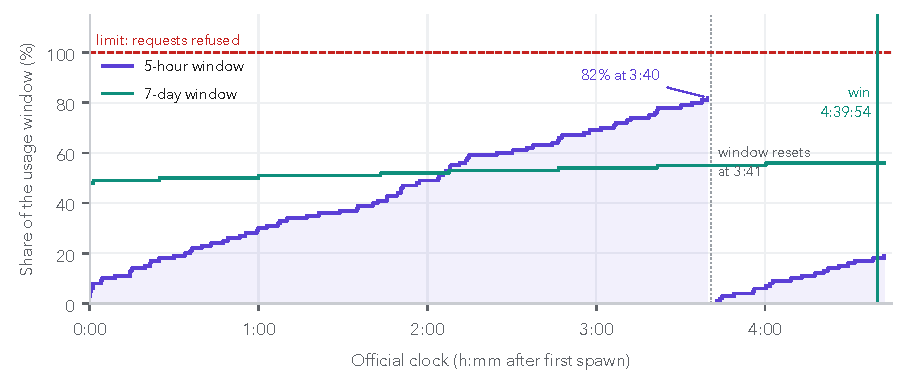
\includegraphics[width=0.9\textwidth]{figures/fig5_usage.pdf}
  \caption{The share of the subscription's usage windows that was spent, at each reading during the run. The 5-hour window stood at 3\% at the first request, reached 82\% at 3:40 and reset at 3:41; the next window stood at 19\% just after the win. The 7-day window went from 48\% to 56\%. No request was refused.}
  \label{fig:usage}
\end{figure}

The 5-hour window rose at about 21 points an hour and never reached its cap. It was within 18 points of it when it reset, at 3:41 on the clock, and the win came 59 minutes into the next window. The reset was luck of timing: the window had opened before the run, so it closed 1 hour 19 minutes before a window opened at the first spawn would have. At the measured rate a single window covering the whole run would have reached about 100\% near the win, so a run this long by one agent at this effort sits at the edge of one window. The account was shared with the planning session, which answered a few short requests during the run; we cannot split the readings between the two.

\section{What the result does not show}
\label{sec:limits}

\begin{itemize}
\item \textbf{The record claim is scoped and unaudited.} It is the fastest time we know of for one AI agent playing alone on a random seed, by this environment's clock and rules, with the block scans and inherited files described here. Faster agent runs are reported outside that scope: 3 hours 56 minutes by one model with 37 ready-made game tools on a chosen seed\footnote{\url{https://huggingface.co/datasets/aibengineering/beat-the-game-minecraft}}, and under 9 minutes by a two-model system on a seed chosen for its supplies and an open End portal\footnote{\url{https://github.com/rmalde/minecraft-agent}}. We did not search for unpublished runs, no outside body keeps such a record, and nobody outside the project has verified this one. The records are kept so that someone can.
\item \textbf{One run, one world.} The fortress was 160 blocks from the portal and a warped forest lay about 330 blocks from the fortress. The benchmark's world had no forest near and a fortress over lava, and the same plan there would have been slower in the Nether.
\item \textbf{Not a comparison of models.} Opus~5.5 has not played this plan, and Fable~5.2 has not played it at a higher effort. The time fell from 6:51 to 4:40 across a change of model, effort, plan and library at once.
\item \textbf{Not blind.} The player read the paper of \citet{faldor2026team}, a plan drawn from five earlier players' records, and their code. Its library began as 4,178 inherited lines and ended at 4,344, beside 1,242 lines of its own one-off programs.
\item \textbf{Block scans.} As in every earlier run, the bot's programs can find blocks through rock. The fortress, the diamonds and the stronghold's frames were all found that way.
\item \textbf{The planner wrote the paper.} The preamble's account of the planning is the planning agent's own. The stage marks and the choice to score the food work as the surprise are judgements made after the result was known; the table gives the numbers both ways.
\item \textbf{The estimate was never tested as an estimate.} A forecast of 50\% needs many runs to check. One win under a 50\% forecast is the most likely single outcome of a well-made forecast and of many badly made ones.
\end{itemize}

\section{What we would change}

\begin{itemize}
\item \textbf{Food is part of every kit and every trip.} Twenty-four meals leave home with the player, and no End entry with fewer than fourteen. Fishing from a sealed pocket is the fallback and takes about a minute a fish.
\item \textbf{Never carry the whole kit on a side trip.} Bows, flint-and-steel and the diamond pick are banked before any trip that is not the main line.
\item \textbf{Build the ring before the first perch.} Once the trench ring around the fountain was finished and the gaze was kept down near endermen, the player took no more damage. Its own estimate with both in place is five perches from full health.
\item \textbf{Fix the model, not just the estimate.} Give the dragon stage and the cost of a death their own uncertainty, let a change work better than estimated, and give each change its own quality instead of one shared knob.
\item \textbf{Repeat it.} The only way to check a 50\% or a 73\% is more runs of the same plan on new random worlds, each one reported.
\end{itemize}

\section{Related work}

Minecraft has long been a testbed for agents, from learned controllers \citep{baker2022vpt,hafner2025dreamer} to language-model agents that write code \citep{wang2024voyager,zhu2023gitm}. \citet{faldor2026team} had teams of agents defeat the dragon, and our earlier papers repeat that with single agents. Agents that keep and reuse what earlier attempts learned are studied as reflection and skill memory \citep{shinn2023reflexion,wang2024awm}; here the memory is a folder of earlier players' files and a plan written from their records. Human speedruns of the same task take minutes \citep{speedrun2026}; the 5-hour goal is a target for this harness, not a claim about that record.

\section{Responsible development}

The agent ran in a sandbox with no network beyond its own game server and the model API, and had no access to the researchers' dashboard. The game was played on a private server. No person other than the operator took part.

\section{Data and code}

The harness, the plan (\texttt{run-5-plan.md}), the odds model (\texttt{scripts/plan-odds.py}) and the frozen prediction with its update script (\texttt{bayes/}) are in the project repository, beside this paper's two scripts: \texttt{run\_data.py} reads the run's records into \texttt{data/run5.json}, and \texttt{make\_figures.py} draws the figures from it. The run is \texttt{2026-11-11-2058}; its observation file for the update is \nolinkurl{bayes/observations/2026-11-11-2058.json}. The planning session's log is kept privately.

\section*{Acknowledgments}

We thank Maxence Faldor, Satinder Singh and Roberta Raileanu, whose paper describes the environment we copied. The plan and this paper were written with Claude Fable~5.2 in Claude Code, in the session the preamble describes.

\bibliographystyle{abbrvnat}
\bibliography{refs}

\end{document}
